\documentclass[border=10pt]{standalone}
\usepackage[svgnames]{xcolor}
\usepackage{amsmath}
\usepackage{pgfplots}
\pgfplotsset{compat=newest}
\usepackage[sfdefault]{FiraSans}
\usepackage{FiraMono}
\renewcommand*\familydefault{\sfdefault}
\begin{document}
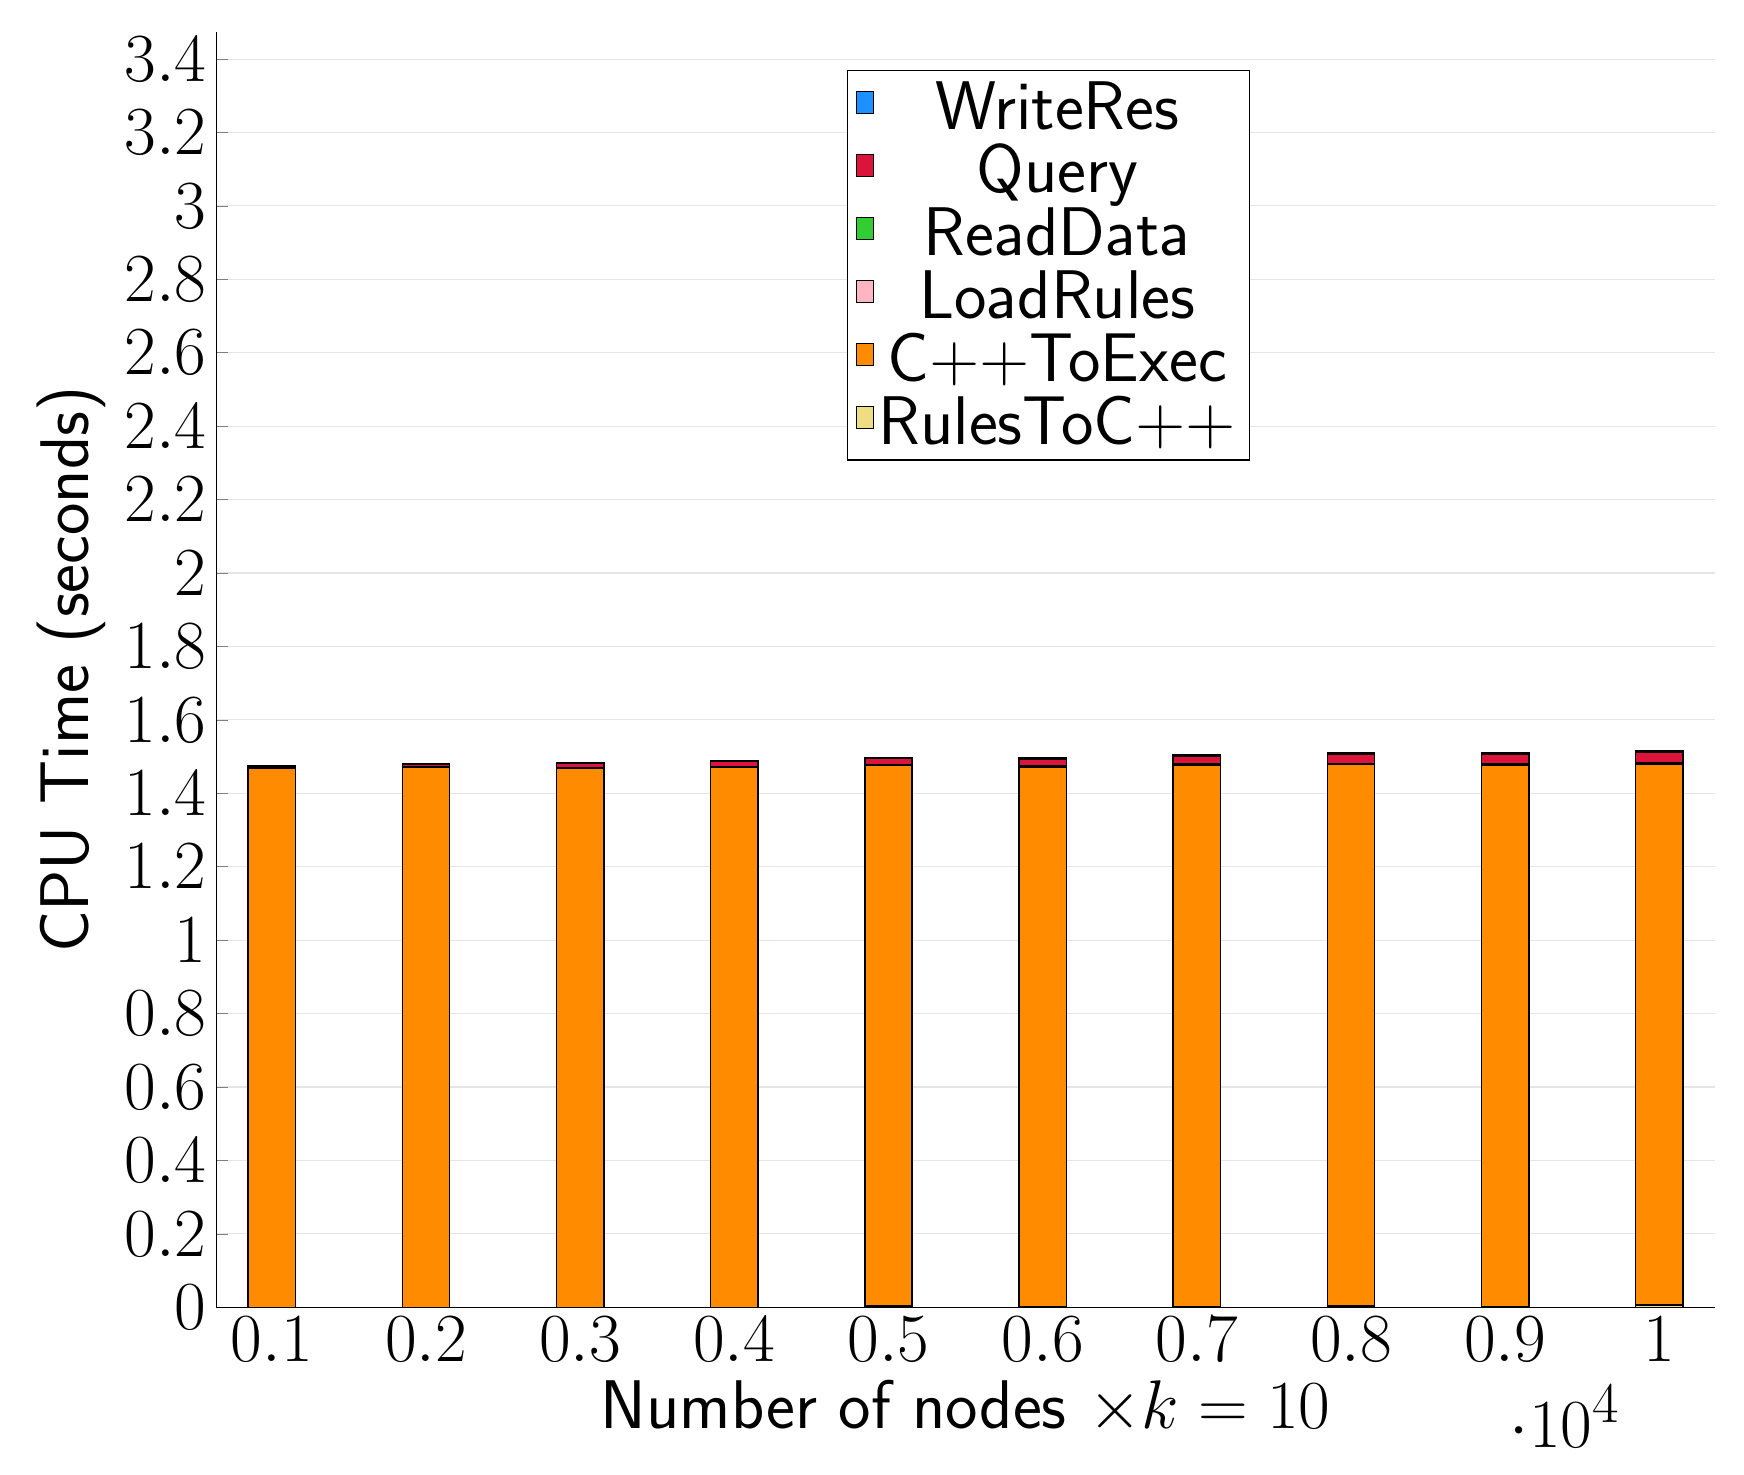
\begin{tikzpicture}
\begin{axis}[
   ybar stacked,
   width=1.7\textwidth,
   bar width=0.6cm,
   ymajorgrids, tick align=inside,
   major grid style={draw=gray!20},
   xtick=data,
   ymin=0, ymax=3.474,
   axis x line*=bottom,
   axis y line*=left,
   enlarge x limits=0.04,
   legend style={
       at={(0.69, 0.97)},
       anchor=north east,
       legend columns=1,
       font=\Huge,
   },
   ylabel={CPU Time (seconds)},
   xlabel={Number of nodes $\times k=10$},
   label style={font=\Huge},
   tick label style={font=\Huge},
]
\addlegendimage{fill=DodgerBlue, draw=black, line width=0.2pt}
\addlegendentry{WriteRes}
\addlegendimage{fill=Crimson, draw=black, line width=0.2pt}
\addlegendentry{Query}
\addlegendimage{fill=LimeGreen, draw=black, line width=0.2pt}
\addlegendentry{ReadData}
\addlegendimage{fill=LightPink, draw=black, line width=0.2pt}
\addlegendentry{LoadRules}
\addlegendimage{fill=DarkOrange, draw=black, line width=0.2pt}
\addlegendentry{C++ToExec}
\addlegendimage{fill=LightGoldenrod, draw=black, line width=0.2pt}
\addlegendentry{RulesToC++}
\addplot +[fill=LightGoldenrod, draw=black, line width=0.55pt] coordinates {
(1000, 0.0)
(2000, 0.0)
(3000, 0.0)
(4000, 0.0)
(5000, 0.004000000000000001)
(6000, 0.0020000000000000005)
(7000, 0.0020000000000000005)
(8000, 0.004000000000000001)
(9000, 0.0020000000000000005)
(10000, 0.006000000000000001)
};
\addplot +[fill=DarkOrange, draw=black, line width=0.55pt] coordinates {
(1000, 1.468)
(2000, 1.472)
(3000, 1.4679999999999997)
(4000, 1.47)
(5000, 1.472)
(6000, 1.47)
(7000, 1.474)
(8000, 1.4739999999999998)
(9000, 1.4740000000000002)
(10000, 1.472)
};
\addplot +[fill=LightPink, draw=black, line width=0.55pt] coordinates {
(1000, 0.0001898)
(2000, 0.00017940000000000002)
(3000, 0.0002038)
(4000, 0.000186)
(5000, 0.00019)
(6000, 0.00020080000000000003)
(7000, 0.00018839999999999997)
(8000, 0.000181)
(9000, 0.0001942)
(10000, 0.0001864)
};
\addplot +[fill=LimeGreen, draw=black, line width=0.55pt] coordinates {
(1000, 0.0008692)
(2000, 0.0011668)
(3000, 0.0017112000000000002)
(4000, 0.0020858)
(5000, 0.0023136)
(6000, 0.0025314)
(7000, 0.0031336000000000003)
(8000, 0.0034881999999999995)
(9000, 0.0039016000000000003)
(10000, 0.004302599999999999)
};
\addplot +[fill=Crimson, draw=black, line width=0.55pt] coordinates {
(1000, 0.0042924)
(2000, 0.0070025999999999994)
(3000, 0.0112494)
(4000, 0.013924200000000001)
(5000, 0.0164656)
(6000, 0.0183762)
(7000, 0.021554)
(8000, 0.0241948)
(9000, 0.025949599999999996)
(10000, 0.0289348)
};
\addplot +[fill=DodgerBlue, draw=black, line width=0.55pt] coordinates {
(1000, 0.0011282)
(2000, 0.0014328000000000001)
(3000, 0.0020244)
(4000, 0.0023206)
(5000, 0.0026784)
(6000, 0.0027099999999999997)
(7000, 0.003194)
(8000, 0.0033589999999999996)
(9000, 0.0036684)
(10000, 0.0038707999999999998)
};
\end{axis}
\end{tikzpicture}

\end{document}
